\documentclass{article}
\usepackage[utf8]{inputenc}
\usepackage[spanish,mexico]{babel}
\usepackage[margin=2.3cm]{geometry}
\usepackage{graphicx}
\usepackage[export]{adjustbox}
\usepackage{caption}
\usepackage{subcaption}
\usepackage{fancyhdr}

\usepackage{listings}
\usepackage{color}

\definecolor{dkgreen}{rgb}{0,0.6,0}
\definecolor{gray}{rgb}{0.5,0.5,0.5}
\definecolor{mauve}{rgb}{0.58,0,0.82}
\lstset{frame=tb,
  language=Java,
  aboveskip=3mm,
  belowskip=3mm,
  showstringspaces=false,
  columns=flexible,
  basicstyle={\small\ttfamily},
  numbers=none,
  numberstyle=\tiny\color{gray},
  keywordstyle=\color{blue},
  commentstyle=\color{dkgreen},
  stringstyle=\color{mauve},
  breaklines=true,
  breakatwhitespace=true,
  tabsize=3
}

\pagestyle{fancy}
\fancyhf{}

\title{Plantilla Facultad de Ciencias, UNAM}
\author{Bruno Iván Cano Velasco}
\author{Jose Ricardo Desales Santos}
\date{\today}

\begin{document}

\thispagestyle{empty}
	
	\begin{figure}[ht]
	   \minipage{0.76\textwidth}
			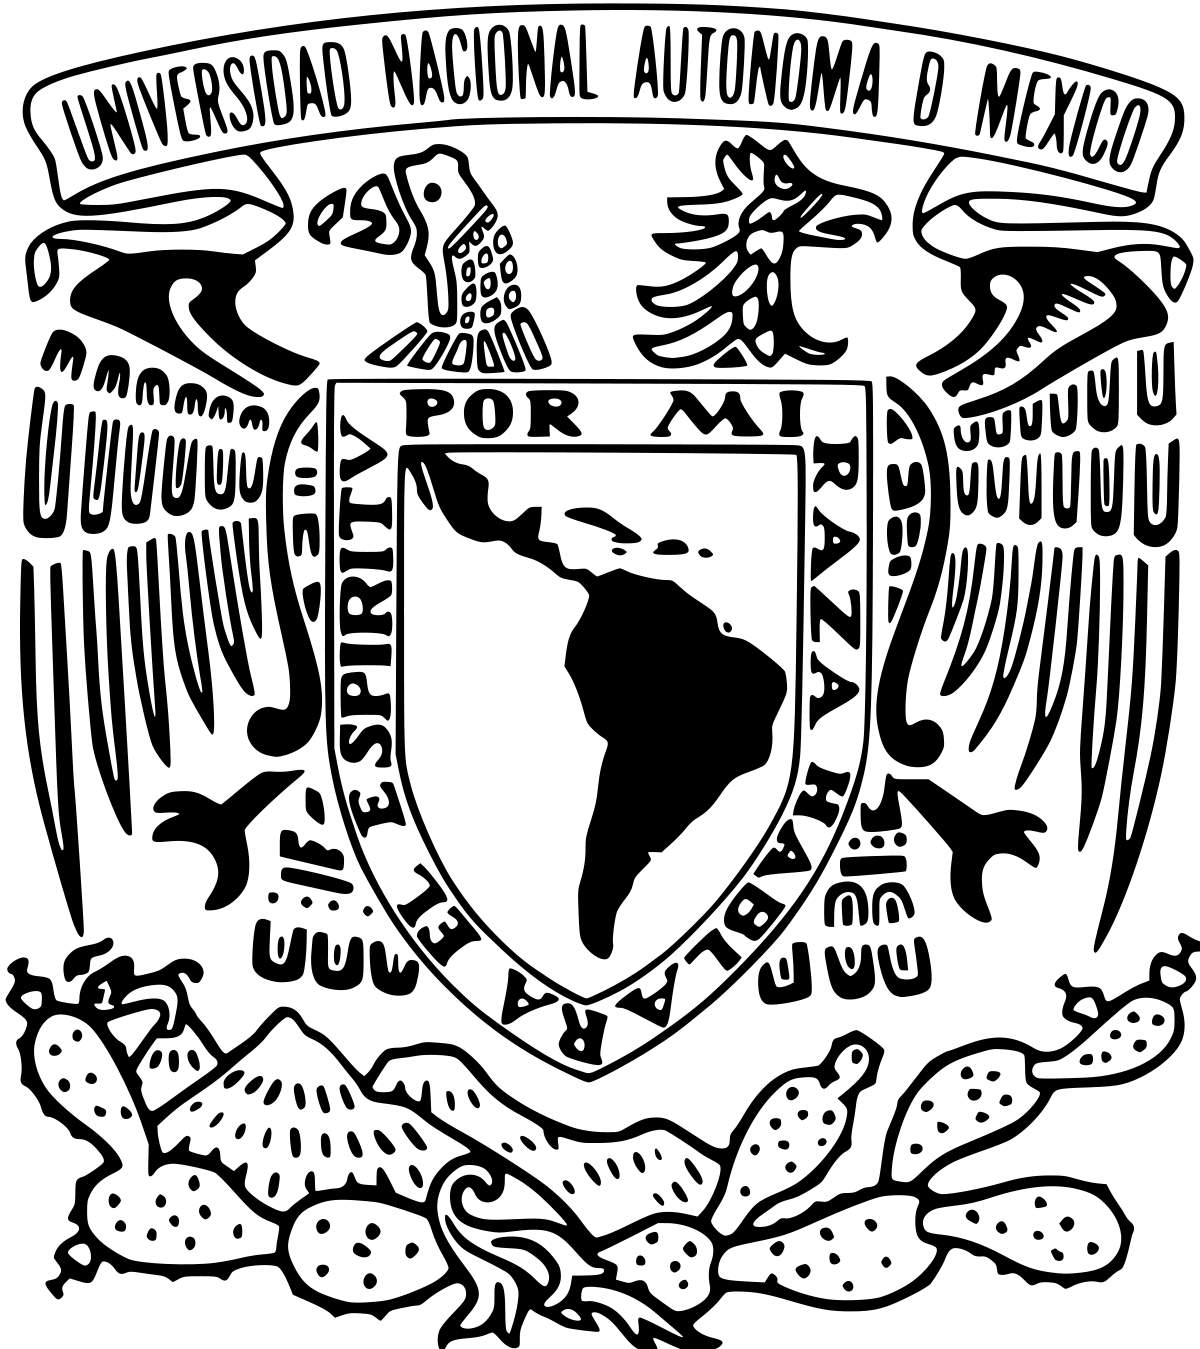
\includegraphics[width=4cm]{assets/Logo_UNAM.png}
			\label{EscudoUNAM}
	   \endminipage
	   \minipage{0.32\textwidth}
			
\includegraphics[height = 4.9cm ,width=4cm]{assets/Logo_FC.png}
			\label{EscudoFC}
		\endminipage
	\end{figure}
	
	\begin{center}
	\vspace{0.8cm}
	\LARGE
	UNIVERSIDAD NACIONAL AUTÓNOMA DE MÉXICO 
	
	\vspace{0.7cm}
	\LARGE
	FACULTAD DE CIENCIAS
	
	\vspace{0.8 cm}	
	\Large
	\textbf{Práctica 1}

	\vspace{0.8 cm}
	\normalsize	
	ALUMNO: \\
	\vspace{.2cm}
	\large
	\textbf{Martin Felipe Espinal Cruces - \texttt{316155362}}
	
	\vspace{1 cm}
	\normalsize	
	PROFESOR \\
	\vspace{.2cm}
	\large
	\textbf{Salvador González Arellano}
	
	\vspace{1 cm}
	AYUDANTES \\
	\vspace{.2cm}
	\large
	\textbf{Rogelio Alcantar Arenas}\\
	\textbf{Eric Toporek Coca}\\
	\textbf{Luis Angel Leyva Castillo}
	\vspace{1.3cm}
	
	\normalsize	
	ASIGNATURA \\
	\vspace{.2cm}
	\large
	\textbf{Computación Concurrente}
	
	\vspace{1 cm}
	\today
	\end{center}
	
	\newpage
	\section*{Pregunta 1}
    \Large 
    ¿Por qué se pone un InterruptedException en el método main?\\
    \normalsize
    Cuando un hilo se encuentra dormido, en espera o en ejecución puede ocurrir que dicho hilo sea interrumpido antes o después de alguna actividad por lo que utilizar la excepción "InterruptedException" lo que nos permitirá cachar el error para evitar terminar el programa abruptamente $^1$
    
    \section*{Pregunta 2}
    \Large 
    ¿Para que sirve el método Join?\\
    \normalsize
    Permite que un subproceso espere hasta que otro subproceso complete su ejecución. A pesar de que es el programador el que decide en que orden poner a esperar un hilo, es decisión del sistema operativo en que momento lo hace por lo que no debe suponer que la esperará exactamente el tiempo que especifique $^2$
    
    \section*{Pregunta 3}
    \Large 
    ¿Qué pasa si no le hacemos Join a los hilos?\\
    \normalsize
    Pondrá a los subprocesos actuales en espera hasta que el o los subproceso en el que se llama esté muerto. Si el subproceso se interrumpe, arrojará InterruptedException. $^2$
    
    \section*{Pregunta 4}
    \Large 
    Explica de manera consisa como usar Hilos extendiendo la clase Thread.\\
    \normalsize
    Creas tu clase extendiendo a la clase Thread. Después tienes que implementar el método run() que será el que ejecuté el hilo. Posteriormente en el método main creas una instancia de tu clase y finalmente a esa instancia llamas al método start() que ejecutará el código que se encuentre en el método run() $^3$
    \begin{lstlisting}
    // Ejemplo
    public class Main extends Thread {
    public static void main(String[] args) {
        Main thread = new Main();
        thread.start();
        System.out.println("This code is outside of the thread");
    }
    public void run() {
        System.out.println("This code is running in a thread");
      }
    }
    \end{lstlisting}
    
    \section*{Pregunta 5}
    \Large 
    ¿Cuáles son las ventajas en implementar Runnable contra extender de Thread?\\
    \normalsize
    La principal ventaja de implementar la interfaz Runnable contra extender la clase Thread es que de esa forma podemos extender de otra clase lo que nos permite mantener la herencia. Cuando extendemos la clase Thread, cada uno de nuestros hilos crea un objeto único y se asocia con él. Cuando implementamos Runnable, comparte el mismo objeto con varios subprocesos. $^4$
    
    \section*{Pregunta 6}
    \Large 
    ¿Se puede predecir el orden en el que se imprimira el mensaje de la clase Hilos?\\
    \normalsize
    No ya que al exisitir múltiples hilos es decisión del Sisitema Operativo o del JVM el orden y tiempo de ejecución de cada uno $^4$
    
    \section*{Pregunta 7}
    \Large 
    En el archivo Hilos2.java, ¿Qué pasa si sacamos la instancia de la clase "h" de $t_1$, es decir, poner h por ejemplo, antes de declar $t_1$?\\
    \normalsize
    Nasa, la ejecución continua sin problema ya que instancia de la clase "h" se utiliza en el método run() 
    
    \section*{Pregunta 8}
    \Large 
    Explica como podriamos tener comportamientos diferentes implementando Runnable\\
    \normalsize
    Si implementaramos la intefaz Runnable tendríamos el método run forzosamente afuera del método main y la instancia de la clase h tendría que estár declarada antes de la instancia de la calse Thread pero en cuenstión de comportamiento serían similares
    
    \section*{Bibliografía}
    \Large 
    \begin{enumerate}
        \item InterruptedException (Java Platform SE 7 ). (s. f.). Docs Oracle. Recuperado 25 de agosto de 2022, de\\ https://docs.oracle.com/javase/7/docs/api/java/lang/InterruptedException.html
        \item GeeksforGeeks. (2021, 17 febrero). Joining Threads in Java. Recuperado 25 de agosto de 2022, de\\ https://www.geeksforgeeks.org/joining-threads-in-java/
        \item Java Threads. (s. f.). W3schools. Recuperado 25 de agosto de 2022, de\\ https://www.w3schools.com/java/java$\_$threads.asp
        \item GeeksforGeeks. (2017, 4 octubre). Implement Runnable vs Extend Thread in Java. Recuperado 25 de agosto de 2022, de\\ https://www.geeksforgeeks.org/implement-runnable-vs-extend-thread-in-java/
    \end{enumerate}
    
\end{document}